\documentclass[12pt]{ociamthesis}  % default square logo 
%\documentclass[12pt,beltcrest]{ociamthesis} % use old belt crest logo
%\documentclass[12pt,shieldcrest]{ociamthesis} % use older shield crest logo

%load any additional packages
%$\usepackage{amssymb}

%input macros (i.e. write your own macros file called mymacros.tex 
%and uncomment the next line)
%\include{mymacros}

\title{Effectiveness of adversarial \\[1ex]     %your thesis title,
       examples on imbalanced \\[1ex] 
       Convolutional Neural Networks}   %note \\[1ex] is a line break in the title

\author{Rafael Carvalhaes Possas}             %your name
\college{School of Information Technologies}  %your college

%\renewcommand{\submittedtext}{change the default text here if needed}
\degree{Master of Information Technology}     %the degree
\degreedate{Sydney, 2017}         %the degree date

%end the preamble and start the document
\begin{document}

%this baselineskip gives sufficient line spacing for an examiner to easily
%markup the thesis with comments
\baselineskip=18pt plus1pt

%set the number of sectioning levels that get number and appear in the contents
\setcounter{secnumdepth}{3}
\setcounter{tocdepth}{3}


\maketitle                  % create a title page from the preamble info
\begin{dedication}
This thesis is dedicated to\\
 someone\\
for some special reason\\
\end{dedication}        % include a dedication.tex file
\begin{acknowledgements}
I would like to express my sincere gratitude to my advisor Dr. Ying Zhou for the continuous support of my master's study and related research. Her guidance helped me in all the time of research and writing of this thesis.

\end{acknowledgements}   % include an acknowledgements.tex file
\begin{abstract}
Convolutional neural networks (CNNs) performance has increased considerably in the last couple of years. However, as with most machine learning methods, these networks suffer from the data imbalance problem - when the underlying training dataset is comprised of an unequal number of samples for each label/class. Such imbalance enforces a phenomena known as domain shift that causes the model to have poor generalisation when presented with previously unseen data. Recent research has focused on a technique called \textit{gradient sign} that intensifies domain shift in CNNs by modifying inputs to deliberately yield erroneous model outputs, while appearing unmodified to human observers. Several commercial systems rely on image recognition techniques to perform well. Therefore, adversarial attacks poses serious threats to their integrity. In this work we present an experimental study that sheds light on the link between adversarial attacks, imbalanced learning and transfer learning. Through a series of experiments we evaluate the \textit{fast gradient sign method} on class imbalanced CNNs, linking model vulnerabilities to the characteristics of its underlying training set and internal model knowledge.

\end{abstract}          % include the abstract

\begin{romanpages}          % start roman page numbering
\tableofcontents            % generate and include a table of contents
\listoffigures              % generate and include a list of figures
\end{romanpages}            % end roman page numberingbishop1995neural

%now include the files of latex for each of the chapters etc
\chapter{Introduction}
Pattern Recognition and Data Mining is a field of study focused on using relatively complex algorithms to discover knowledge from large pools of data. These are used to predict the future or to recognise patterns and label data points that are close together. The increase of computational power on the last two decades leveraged the use of techniques such as Neural Networks \cite{bishop1995neural} to tackle more complex problems like automatic labeling of digital images. The work of Lecun (1989) \cite{lecunn89} was one of the stepping stones for all work on image recognition using Neural Networks as he was able to prove the effectiveness of stacking multiple layers of neurons to form what we call a Neural Network. These studies usually refer to how the human brain works to explain the inspiration of such techniques and each neuron was later named as perceptrons.

The focus on the early days of neural networks was to understand the main principles behind human learning. For instance, recognizing handwritten digits could be seen as a trivial and effortless job for most people, however, making a computer to be able to perform this same task was not as easy as it seemed. By discovering the pattern behind digit recognition, computers would also be able to start understanding broader classes of images \cite{krizhevsky2012}. The use of computer vision techniques along with machine learning algorithms are nowadays the state of the art techniques to overcome these challenges.

Computer Vision is a field of study that focuses on processing digital images and has Neural Networks as one of the most used predictive techniques. These algorithms are focused on learning models that recognise patterns on data with several dimensions (e.g. images with width x height number of pixels). Recent advancements on both Computer Vision and Neural Networks have led to the development of a new class of algorithms which is nowadays known as either Deep Learning or Deep Feed Forward Networks.

Extremely deep networks (e.g. one containing stacked perceptrons layers) are categorized as deep learning algorithms and can be more popularly represented through deep feed forward neural networks \cite{hornik1989multilayer} and, more recently, recursive neural networks \cite{goller1996learning}. While the latter focuses on solving problems where data points are dependent on one another (e.g. Time series) the first is more largely used on image recognition and, therefore, should be the focus of this work. A more specific approach on deep feed forward nets is to extract important features from images before trying to classify them as a predefined class. This approach is widely used on a specific Neural Network architecture called Convolutional Neural Networks (CNNs) \cite{matsugu2003subject}.

Recent work has shown that the generalization learned into DNN's networks is rather sparse \cite{goodfellow2016}. This sparsity enables methods to intentionally fool the network into predicting a different class for a given image. This operation is comprised of changing current images by adding just enough directed noise to each pixel in order to fool an algorithm into thinking that the image has a different label \cite{goodfellow2014}\cite{papernot2016transf}\cite{goodfellow2016}\cite{szegedy2013}. The resulting images of this process are known as Adversarial Examples and their generation can be mainly done through the use of a method called Gradient Sign \cite{goodfellow2014}.

The imbalanced learning is a well known cause for lower performance of several machine learning algorithms. Data distribution on real world is usually skewed and rarely contains enough information to learn all the necessary features of the data domain. As the dependency of specific class labels grows, the vulnerability of the system increases, as wrong predictions of the critical label could lead to unwanted outcomes. Adversarial examples are known for forcing domain shift on classes with similar distributions and, hence, are able to change the classification labels of test inputs. The imbalanced class problem could then become more critical when the use of such technique happens to models where the data domain presents the aforementioned characteristics.

This thesis presents an experimental approach aimed to understand the factors leading to the robustness to adversarial attacks of  class imbalanced Convolutional Neural Networks. Through the use of the Fast Gradient Sign Method we investigate how a skewed data distribution could affect the network robustness to such attacks. Understanding such threat vectors is of the utmost importance for the development of current techniques, as it drives the creation of new regularization techniques.


\section{Motivation}

To date, little evidence has been found associating training characteristics of a model with its robustness to adversarial examples. Experimental demonstrations of adversarial effects were carried out mainly by the deep learning and computer vision community. The motivation for Adversarial robustness comes largely from being able to shield image recognition systems from behaving unexpectedly. Previous published studies are limited to showing the general effectiveness of adversarial methods rather then understanding the deep relationship with the underlying training data distribution.

The world is embracing Artificial Intelligence and there are already a large number of solutions that rely on image recognition algorithms to perform tasks that range from car plate recognition to more general machine learning APIs such as Amazon Rekognition. In particular, computer vision and up to date machine learning algorithms could greatly benefit from understanding the relationship between the imbalanced learning problem and adversarial attacks.

\section{Thesis Goals}
This study is set out to provide evidence on how models trained on skewed distributions could be more or less vulnerable to adversarial attacks. The main contributions of this work are as follows:
\begin{itemize}
	\item To shed new light on how the domain shift caused by adversaries is affected by imbalanced feature space exploration on Deep Neural Networks
	\item To fill gaps on literature regarding adversarial examples impacts on CNNs and how one could possibly increase the robustness to these attacks for specific class labels
	\item To specifically enhance understanding of Convolutional Neural Networks vulnerabilities and its implications to real world scenarios.
\end{itemize}

\section{Thesis Structure}

This thesis first gives a brief overview of the recent history of Neural Networks and the main related techniques and methods for using such networks on computer vision related tasks. Next chapter begins by introducing all the taxonomy around Adversarial Examples followed by a theoretical discussion of domain shift in machine learning. Lastly it presents two variations of the gradient sign method and its different perturbation types. The fourth chapter presents an empirical study of machine learning transferability and provides a practical overview of different attacks to real world systems. The remaining chapters are concerned with explaining the experiment setup and presenting the achieved results and related future work.

\chapter{Background}

This chapter provides a review of the current research on Deep Neural Networks, their optimization techniques and the state of art results for image recognition. Optimization methods will be first discussed followed by current DNN architectures.

\section{ (Shallow) Neural Networks}

In the context of machine learning, Neural Networks are a class of differentiable algorithms \cite{bishop1995neural}. One can think of them as a set of perceptrons aligned into several layers having outputs from layer \textit{L} mapped to inputs of the layers \textit{L+1}. The output of each perceptron is named activation and the set of activations in the final layer gives the desired classification output. For each connection, a neuron has one weight connecting with all neurons of the next/previous layer, and one bias. The goal is to find the values that minimizes a given cost function. For instance a network could have 10 neurons in the last layer that would map to a digit classification problem using the MNIST \cite{lecun1998mnist} dataset. The neurons from 1-10 on this layer corresponds to each number, and the one with the highest activation value would be chosen as the classification output.

\begin{figure}[h!]
\centering
	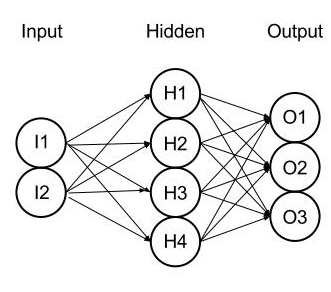
\includegraphics[scale=0.5]{mlnet.png}
\caption{Multi-layer Perceptron}
\label{fig:mlnet}
\end{figure}


\section{Gradient Methods and Backpropagation}

As most machine learning algorithms, Neural Networks models rely on optimizations of weights $\omega$ and biases $\beta$. In order to calculate these values one should  choose a cost function that measures the variance between the actual result and the desired output on each iteration of the training phase. The two methods for running this optimization algorithm on Neural Networks are known as \textit{Backpropagation} and \textit{Gradient Descent} \cite{goodfellow2016_book}. The main goal of the algorithm is to propagate small changes $\delta$ applied to any of the neurons of the network all the way to the final layer.

\begin{figure}[h!]
\centering
	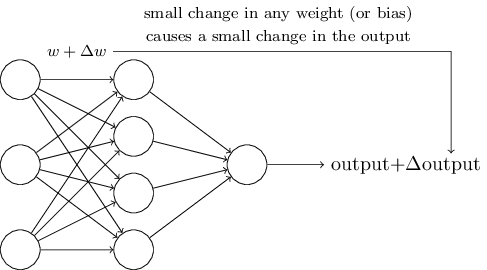
\includegraphics[scale=0.5]{net_change.png}
\caption{Output change with regards to layer(s) weight change \cite{nielsen2016}}
\label{fig:net_change}
\end{figure}


The network learns from data using convex optimization techniques that involves calculating derivatives of linear and polynomial cost functions.The learning algorithm should be able to find weights and biases that best approximates the output \textit{y(x)}. This approximation consists of finding the global minimum of a chosen cost function. Different machine learning algorithms require different cost functions \cite{nielsen2016}. Ultimately, one should be interested in calculating the change on the cost with respect to the weights and biases of all the neurons. This calculation makes use of partial derivatives with respect to the $\omega$ and $\beta$ in order to find the direction of the minimum for a given function $f(x)$, namely gradient \cite{goodfellow2016_book}.

$$\nabla C \equiv \frac{\partial C}{\partial \omega}, \frac{\partial C}{\partial b}$$

Gradient Descent is one of the methods for finding a global/local minimum of a function. This calculation yields what is a called a gradient vector $\nabla$C which is subtracted from current weight and biases on each iteration in order to move the result towards the global or local minimum. The gradient calculation can be seen as repeatedly computing $\nabla$C, and then moving in the opposite direction "falling down" the slope of the valley.

\begin{figure}[!ht]
\centering
	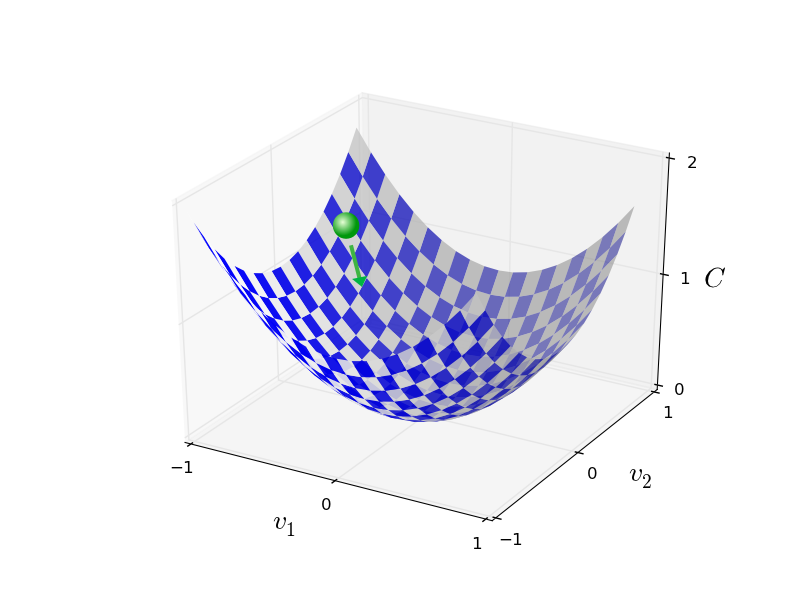
\includegraphics[scale=0.3]{valley_with_ball.png}
\caption{Gradient calculation representation \cite{nielsen2016}}
\label{fig:net_change}
\end{figure}
In order to learn the best representation of a given data set a Neural Network should go through the optimization process where each data point is used many times to estimate the network current weights and biases. Each iteration pushes the ball into the direction of the valley by comparing a given y($x_n$) with its corresponding real $y_n$. The process should be stopped when the ball hits the lowest point of the valley, in other words, when the algorithm has converged. Mathematically speaking this is known as reaching a minimum of a function \cite{nielsen2016}. Some optimization problems are unable to find a global minimum due to their complexity, on this case, convergence is achieved by finding the local minimum.

However, when the data set is too big for running one update after a complete loop over the entire data, one should come with better strategy for updating the network parameters. Such method is that where each iteration runs on a subset of the training input namely \textit{Stochastic Gradient Descent}. One of the biggest advantages is that to speed up learning while the estimation of the gradient $\nabla$C is being computed over a subset of the data instead of all training inputs. The subset is chosen randomly on every iteration and can be referred as mini-batch. These batches are selected every \textit{epoch} and the user provides how many epochs the algorithm should run. Due to the large amount of parameters, neural networks used in Deep Learning make use of this method so training can happen within feasible time frames.


The training is comprised mainly of two different types of calculations: Feedforward and Backpropagation. Feedforward is the starting point of the network weights and biases optimization.The goal is to calculate the activation of each neuron from the first layer to the output layer. It involves evaluating the activation function with respect to the current weights and biases of the network by forward-propagating \textit{x} through the entire architecture. This operations yields an error $\delta$, which triggers the backpropagation part. When feedforward reaches the last layer, the error is then calculated and backpropagated to the L-1 layer. For each layer, one should find the rate of change of the cost function for each of the weights and biases with respect to its neurons. This operation is repeated subsequently until the first input layer, where the current "belief" of the network is updated making it ready for another feedforward calculation. The overall process should stop when there is no relevant changes in the output of the cost function.

\section{Convolutional Neural Networks}

Convolutional Networks are a class of deep learning algorithms that can use many layers of nonlinear or linear processing in cascade for feature extraction and transformation. They are still very similar to ordinary Neural Networks (made up of neurons that have learnable weights and biases). However, such algorithms makes the explicit assumption that the inputs are images and, therefore, are based on learning abstract representations of data with spatial properties \cite{goodfellow2016_book}. For example, an image could be represented by a vector of intensity values from 0-255 for each pixel and after being processed by the first layers of a Convolutional Neural Network those would become more abstract representation such as set of edges, regions of particular shape and etc \cite{stanford2016}.

A convolutional neural network is different from the traditional neural network. Instead of connecting each pixel of an image, for instance, to all the neurons in the next layer, groups of pixels of fixed sizes known as patches, are connected to different groups of neurons. Each group specializes in learning specific features from the data and are not necessarily connected with all other groups in the current or next layer. The input region or group of neurons connected to a patch in the image is known as local receptive field \cite{nielsen2016}. The main advantage over shallow architectures is that the latter does not take into account the inherent spatial structure of images, in other words, all pixels are treated equally.

The main architectural difference of ConvNets is that they have added some different layers to the traditional Neural Nets mix. The name "convolutional" originates from the Convolution layer which is responsible for computing the output of neurons that are connected to local regions in the input. This operation is commonly referred in image/signal processing as a convolution between two matrices/vectors of variable sizes. The smaller regions in which the image is connected is referred as filters and/or kernels, and these would be responsible for detecting abstract features on different regions of a picture for instance. After each sequence of convolutional layers there are also the Pooling Layers. The main goal is to perform downsampling operation along spatial dimensions of an image (i.e width and height). This is important as an image with higher dimensions will be reduced at each layer forcing the network to learn deeper and deeper features at each iteration.

\begin{figure}[!h]
\centering
	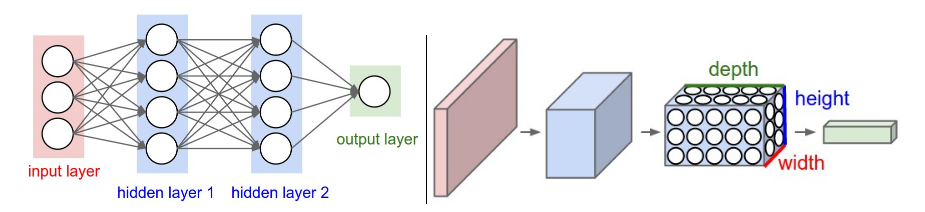
\includegraphics[scale=0.6]{conv.png}
\caption{Shallow Neural Network vs Convolutional Neural Network}
\cite{stanford2016}
\label{fig:conv}
\end{figure}

Convolutional Neural Networks are considered the state of the art solution for computer vision problems. The archutecture developed by Krizhevsk et al. (2012) achieved an averaged top-1 and top-5 test set error rates of 37.5\% and 17\% where the previously record was 45.7\% and 25.7\% by a different technique. The network was comprised of eight layers, 5 of which were convolutional layers and the remaining were three fully connected layers. The output of the three last layers was fed to a 1000-way softmax to produce 1000 different image classes labels of the ImageNet dataset. Besides, max-pooling layers were also used following the fifth convolutional layer and response-normalization layers. Adding or removing any layers on this architecture yielded worst results. Overfitting was treated by using both Data Augmentation and Dropout \cite{hinton2012improving} techniques since the architecture had over 60 million parameters. These results show that deep convolutional networks are capable of achieving above the average results even when challenging datasets with several classes are used.
\section{CNN Feature Learning and Visualization}

Visualizing the features of a convolutional layer helps one to understand what are the main characteristics of the input that are not only being learned but are also responsible for maximizing neurons activations cite{zeiler2014visualizing}. Until recently there was no clear understanding of why Convolutional Networks perform so well on image classification tasks. Zeiler et al (2014) have produced a novel visualization technique that gives insights into the outputs of the intermediate feature layers of the network. These visualizations were then used to perform diagnostics of models and, thus, find architectures that can outperform current state of the art algorithms. One can understand that all the convolutional layers are in fact "feature extraction" layers while the fully connected ones are the actual classifier.

\begin{figure}[!h]
	\centering
	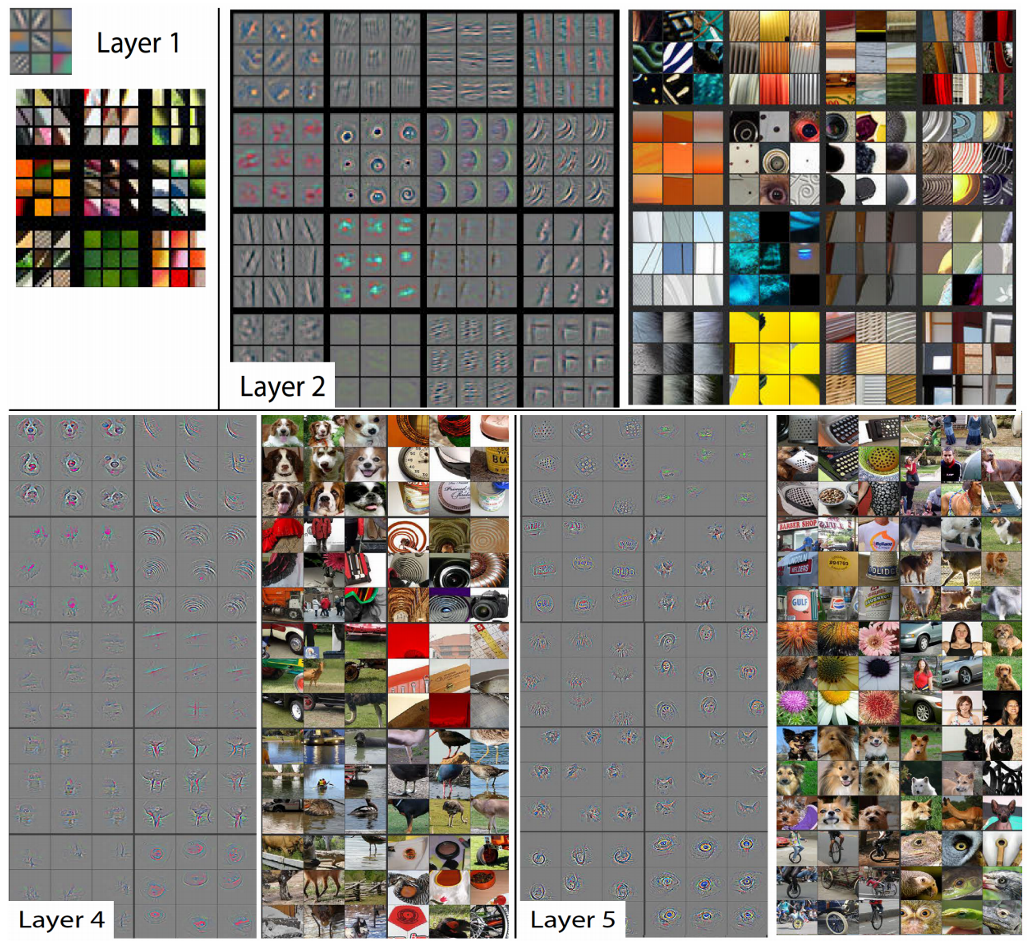
\includegraphics[scale=0.6]{layer_vis.png}
	\caption{CNN layer visualization}
	\cite{zeiler2014visualizing}
	\label{fig:conv_layer_vis}
\end{figure}

Features are learned from more abstract on initial layers to more specific and concrete on deeper layers. Figure ~\ref{fig:conv_layer_vis} shows that the first neurons are learning different types of edges while later neurons are capable of learning full representations of important regions of an image. In general these features are applicable to many datasets and tasks. As features transition from general to specific, transferability becomes negatively affected \cite{yosinski2014transferable}. For instance two similar datasets as the ImageNet and Cifar10 would share many common features and, therefore, a network trained on one, could be used as a pre training or weight initialization process for another, increasing the generalization and accuracy of the model.
\section{CNN Architectures}

The use of Deep Neural Networks (DNNs) as a prominent technique was mainly possible due to the standardization of the dataset used for such tasks. ImageNet has become the most used classification challenge for those wanting to find better CNN architectures. The main goal of such challenges are to find models with better accuracies without focusing too much on resource utilisation. One one hand, the most important metric of a good machine learning model is its accuracy, in other words, how well it can generalize on different datasets. On the other hand, several other important metrics should be taken into consideration when using an specific DNN system in real life such as: memory footprint, parameters, operations count and etc \cite{canziani2016analysis}.

\begin{figure}[!h]
	\centering
	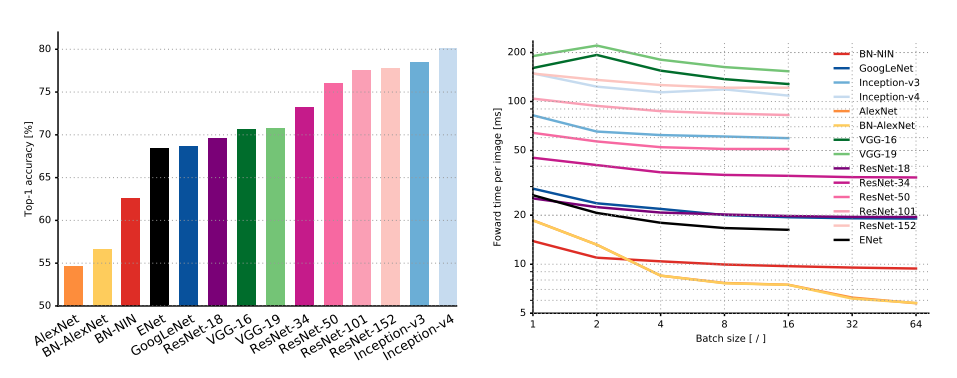
\includegraphics[scale=0.6]{network_comparison.png}
	\caption{(Left) Accuracy of Different CNN models (Right) Inference time for different batch sizes}
	\cite{canziani2016analysis}
	\label{fig:cnn_comparison}
\end{figure}

As new methods develop, one should always pick the one that is capable of not only learning the features of the target domain but also would fit the resource capacity of the system. From one of the first CNN architectures (AlexNet) to the latest models (Inception V4), the accuracy has improved from $55\%$ to almost $80\%$ on the ImageNet dataset (comprised of 1.000 different class labels).

\section{Deep Neural Networks Properties}\label{subsec: nn_props}

Deep Neural networks can be considered models with high expressiveness that can achieve extremely good performance on computer vision tasks. At the same time that being highly expressive helps them to succeed, it also drives them to learn solutions that are not easily understandable \cite{szegedy2013}. Usually there is a discontinuity in the input-output mappings of neural networks which can lead to miss-classification of images when the network prediction error is maximized \cite{gu2014}.The learning process of these networks through the use of backpropagation is rather complex and sometimes difficult to understand.

In order to visualize the semantic meaning of individual units, studies are currently focusing on understanding the factors leading to the activation of network neurons. It has been argued that deep neural networks should be stable enough to provide robustness to small perturbation of its inputs \cite{szegedy2013}. However, it has been found by mainly Goodfellow et al. (2014) and Szegedy et al. (2013) that minimal local perturbations can indeed affect the network's predictions bringing down the assumption that DNN have very good local generalization. Methods for exploiting this vulnerability were created and proven to be effective by having a very high confidence classification of adversarial examples \cite{goodfellow2016}.

Generalization is usually achieved by making non-local assumptions of the training inputs. Deep stacks of non-linear layers are one of the ways to have the model encoding a non-local generalization prior over the input space \cite{gu2014}. Therefore, output units should be able to assign low probabilities to regions of the input space where no training examples are found within its vicinity. The representation of low-probability "pockets" of space on images can lead to the creation of Adversarial examples. These are created by adding small localized perturbations on the input space which can ultimately lead to the wrong classifier outcome. 


The following sections are going to focus on Adversarial Examples and how the exploitation of the aforementioned network properties can be used to craft such examples. Three methods will be presented along with results found by different studies. Finally, methods for using this adversarial information for regularizing networks will also be shown as a possible solution for making deep neural networks less vulnerable to these kind of attacks.

\chapter{Adversarial Examples Taxonomy}

This chapter focuses on Adversarial Crafting and how these examples can be used to exploit some of the Deep Neural Networks caveats seen in the last chapter. Firstly the Fast Gradient Sign method will be explained along with some results. Secondly, a brief discussion on the empty pockets of space created by neural networks allow such technique to create adversarial. Finally a discussion of the potential threats these pose to systems relying on machine learning algorithms to perform their tasks.


\section{Foundations}

Understanding of why adversarial samples can exist requires exploration of how learning models are built. The training data is a corpus of samples taken from a expected input distribution and are labeled accordingly to their desired class. For instance, this sample data would be a large number of emails or a huge data set of images. The labels are then taken as ground truth when constructing models to be used at runtime.

The integrity of deep learning systems usually is that of that measures how accurate the system is when performing a classification task. This metric is of paramount importance and, therefore, should be a common target for techniques trying to exploit such algorithms vulnerabilities. Specifically, an adversary of a deep learning system seeks to provide an input X' that results in incorrect output classification. The incorrectness of the prediction can be represented into different natures and can impact the classifier output in different ways.

Adversary drivers could be explained into four goals as discussed by Papernot(2016) \cite{papernot_thesis_2016}. Confidence reduction is the adversary potential to introduce class ambiguity by reducing classification confidence. Misclassification happens when a label of the model being previously correct is changed to an incorrect output label. On the same way, one could use a Targeted misclassification to produce inputs that forces outputs into a specific label. Finally, the source/target misclassification forces the output classification of a specific input to be a specific target class.

\section{Domain Shift}

Regardless of the technique, a machine learning model represents an approximation of the phenomena being modeled. In most cases the training data is unable to represent all possible input feature vectors and, therefore, can not full capture a complete understanding of the target domain. A problem arises when input examples are able to exploit the system by providing samples that are not within the aforementioned input domain. They usually use information about the system to find where the model is inaccurate owing to missing items of the given training set.

Classification accuracy should be carefully measured when training a model. For instance, the value of the training set is usually higher than the one on the test set. This happens when the samples of the training can not cover the entire data distribution space and therefore the domain covered differs from the one on the test set. A poor performance on the test set means that the divergence of both distributions (training and test domains) is high. 

What adversaries do is to force the domain shift in a way that the model is unable to generalize well on test data. Since data in almost circumstances can not cover the entire feature space, the real decision boundary of a classification model generally becomes more complex as the phenomenon becomes more nuanced and the feature and dimension space becomes larger. This complexity is exploited by adversaries through the use of the model error as a guideline for perturbing a sample.

\begin{figure}[!h]
\centering
	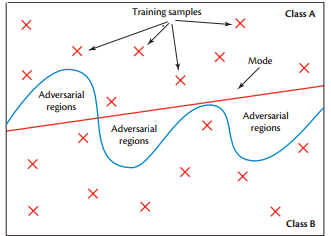
\includegraphics[scale=1.0]{adv_space.png}
\caption{Two Dimensional Representation of unexplored adversarial regions \cite{papernot_2017}}
\label{fig:adv_space}
\end{figure}

\section{Fast Gradient Sign}

The Fast Gradient Signed method developed by Goodfellow et al. (2014) has been used as the foundation of many of the experiments in adversarial crafting. The results have led to the hypothesis that DNNs can possibly have linear behavior when in very high dimensional space.  Most inputs were miss-classified not only on Goodfellow et. al \cite{goodfellow2014}  experiments but many other. This shows that adversarial examples are not hard to find. The method consists on using gradient information to generate image noises that changes classification outputs.

$$ C(x + \delta)\approx C(x) + \delta * \nabla C$$

The equation aims into adding noise that emphasizes the pixels in the image with the highest importance, so the resulting perturbation can likely lead to a misclassified result. By using the \textit(sign) function of the gradient, it is assured that the value will grow linearly with the number of the dimensions \cite{goodfellow2014}. The result of many small pixel changes is likely to generate an image with a wrong label in the network output.

$$ C(x + \delta)\approx C(x) + \delta * sign(\nabla C)$$

Billovits et al (2016) categorized four different categories of adversarials generated by FGSM. True Adversarial are those given a completely different label after being perturbed. Re-Focused adversarial is the method that changes the focus of an image by giving a classification of an object that used to have lower significance while keeping the original object presence. Conaturally Adversarial are those where the new output has some close relation to the miss-classified result (e.g. Dog and Cat). Finally, Benign adversarial hapeens when neural networks misses the top prediction of the original image but the adversarial example gets classified correctly with high confidence \cite{billovits}.

\begin{figure}[!h]
\centering
	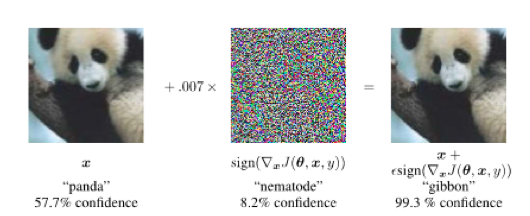
\includegraphics[scale=0.6]{panda.png}
\caption{Adversarial example crafting with fast gradient sign \cite{goodfellow2014}.}
\label{fig:fgsm_craft}
\end{figure}

\section{Unrecognizable Images}\label{subsec:unrec}

Adversaries, on the other hand, are not only comprised of small perturbations on known images. Nguyen et al (2015) presented a method for producing images that are unrecognizable to humans, but are nonetheless labeled as recognizable objects by DNNs \cite{nguyen2015}. For instance, a DNN would classify a noise-filled image crafted using their technique with high confidence. These images were named $fooling images$ since they do not have a source class but are crafted solely to perform a targeted misclassification attack.

\begin{figure}[!h]
\centering
	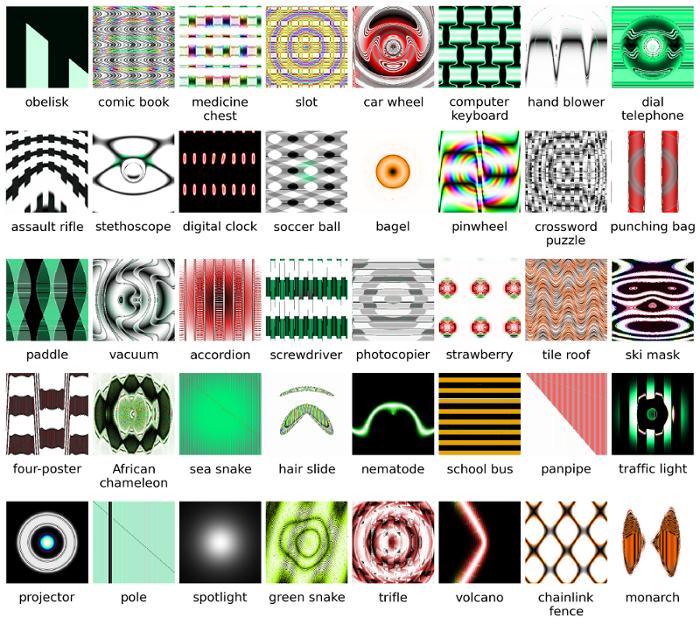
\includegraphics[scale=1.]{unrec_images.png}
\caption{Examples of noisy images classified with high confidence \cite{nguyen2015}.}
\label{fig:unrec_images}
\end{figure}


\section{Adversarials in the Physical World}\label{sec:physical}

All the aforementioned techniques were based into feeding information directly into machine learning systems. Such model only takes into consideration situations in which attacks take place entirely within the computer. For instance, these techniques could be used by attackers to avoid spam filters or malware detectors. Even though the study is utterly relevant, a recent study conducted by \cite{goodfellow2016} have shown that it is possible to craft adversarial samples in order to perform attacks on machine learning systems which are operating in the physical world.

Although the Fast Gradient Sign method have been successful on crafting adversarial examples, there are some extensions of the method that can be used in order to create perturbations that are more likely to work in the physical world. Firstly, \cite{goodfellow2016} introduced a variation named \textit{Basic Iterative Method}. This technique consists of applying the fast method multiple times with small step sizes and making sure that all pixels are within a $\epsilon$-neighbourhood of the original image. The number of iterations was chosen heuristically with goals of being sufficient enough to have the adversarial example reaching the edge of the $\epsilon$ max-norm.

In order to perform experiments, clean photos of adversarial examples created using the three methods were taken and fed into a machine learning system using Deep Convolutional Neural Networks (Inception V3). Adversarial Images created using the "fast" method were more robust when compared to the iterative methods. The hypothesis behind the result is that iterative methods create more subtle perturbations that can be easily be destroyed by the photo transformation process (Photo Printing as described above). Overall, it could be expected that about 2/3 of the images would be top-1 misclassified and about 1/3 top-5 misclassified by the fast method using an $\epsilon$ of 16.

Adversarial examples is not only feasible on digital attacks but also on physical world scenarios. By using the correct perturbation algorithm with optimized hyperparameters one can use printed digital photos to fool day-to-day machine learning systems. As more and more machine learning is becoming part of our environment, techniques for avoiding such attacks need to be developed so these systems can become less vulnerable to any kind of attack.
\chapter{Attacking Machine Learning Systems}

In this chapter, we present approaches for attacking machine learning algorithms with adversarial techniques presented in the previous chapter. We discuss that the knowledge of the architecture and weight parameters is sufficient to derive adversarial samples against DNNs. Further discussion goes into black box attacks where the attack has minimal information about the underlying system. The discussion is then concluded with how model's knowledge can be transferred between different algorithms/techniques.


\section{Transferability}

Papernot (2015) presented that many adversarial examples crafted to fool one specific model are also likely to affect another different model. As long as the models were trained to perform the same task, knowledge can be transferred when querying the victim model, namely oracle, to label a synthetic training set for the substitute.

The machine learning transferability property constitutes a threat vector for many state of the art methods, thus, one should be able to quantify most vulnerable classes of models by generating accurate comparison of the vulnerabilities of each class. Attacks can, however, depend on some specific information of the target as shown in Table ~\ref{tbl:attack_info}. Techniques can mainly be split into both Intra-Technique and Cross-Technique. These are discussed in more details on the following sections.

\vskip 1cm

\begin {table}
\begin{tabular}{|c|c|}
	\hline 
	Model Parameters (Weights and Biases) & Have full access to model wieghts \\ 
	\hline 
	Model Architecture / Type & Know what the model looks like \\ 
	\hline 
	Training data & Understand the data domain \\ 
	\hline 
	Oracle/Black box & Query model with input X, get label Y \\ 
	\hline 
	
\end{tabular} 
\caption {How Much Information is needed to fool a model?}
\label{tbl:attack_info}
\end {table}

\medskip



\section{Intra-technique transferability}\label{sec:intra}

The Intra-technique transferability is achieved by reproducing the learning process between two identical algorithms \cite{papernot2016transf}. Even though, the algorithms can differ in terms of architecture, they are still based on the same fundamental learning concept. For example, most learning algorithms could be categorized into three general classes: differentiable algorithms like DNN and Logistic regressions, lazy learners like KNN and non-differentiable models like SVM and Decision Trees. Therefore, this technique consists of keeping the same learning method while differing the hyperparameters/architecture and using queried subset of the training data to train the local model. 



In order to make a comparison between these techniques, Papernot N. et. al (2015) \cite{papernot2016transf} created five different dataset models of the MNIST to train the algorithms and compare how they perform when using different and same models of training data. All models had non-negligible vulnerability to this kind of approach. While DNN and LR were highly vulnerable to these attacks, SVM, DT and KNN were more robust achieving better overall resilience. The results have led to the hypothesis that non-differentiable techniques are more robust to black-box attacks using locally generated adversarial sample with two algorithms of the same type \cite{papernot2016}. Figure ~\ref{fig:intra} shows classification performance when using intra-technique methods.

\begin{figure}[!h]
\centering
	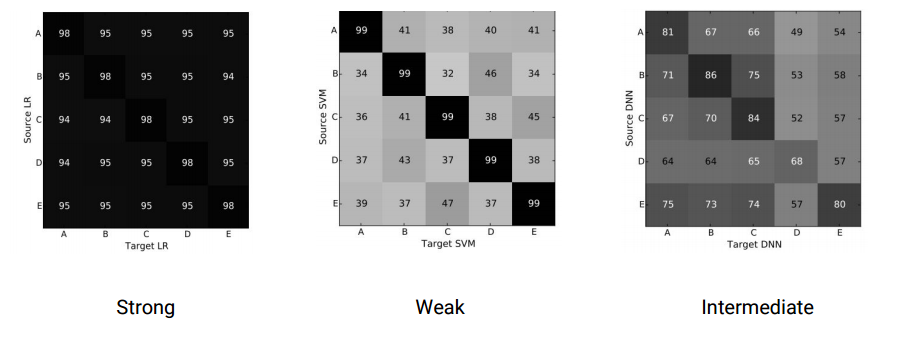
\includegraphics[scale=0.6]{intra.png}
\caption{Knowledge transfer level using Intra-Technique Transferability \cite{papernot2016transf}}
\label{fig:intra}
\end{figure}


\section{Cross-technique transferability}
Cross-Technique transferability was referred as the knowledge transfer between two different machine learning techniques. This technique has a higher degree of difficulty than the method shown on section \ref{sec:intra} as it involves models using possibly very different techniques like DNNs and Decision trees. Yet, this can be seen as quite strong phenomenon to which techniques like Logistic Regression, Support Vector Machines and Decision Trees along with Ensemble based models are extremely vulnerable \cite{papernot2016transf}.

Papernot N. et. al \cite{papernot2016transf} have shown a strong but not linear phenomenon. While DNN's ended up as being the most robust of the methods with misclassification rates varying between 0.82\% and 38.27\%, Decision Trees were the most vulnerable with rates from 47.20\% to 89.29\%. Interesting enough, ensemble methods -- focused on measuring the output of all the "experts" in the group -- have shown quite vulnerable to the experiment. The hypothesis is that the technique explores the individual vulnerability within each of the ensemble methods.

\begin{figure}[!h]
\centering
	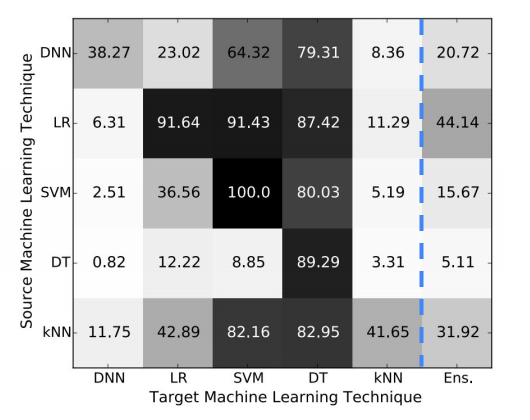
\includegraphics[scale=0.6]{cross.png}
\caption{Knowledge transfer using Cross-Technique Transferability and Ensemble Methods \cite{papernot2016transf}}
\label{fig:cross}
\end{figure}
\section{Black-box Attacks}
Black-Box attack to machine learning systems alleviates the dependence on knowing both victims training data and model information. This method solely depends on accessing the label assigned by the target for any chosen input. The strategy consists of learning a substitute for the target model using a synthetic dataset generated by the adversary and labeled by the observed victim, namely here, the Oracle \cite{papernot2016}.

Training the substitute model that approximates the Oracle poses some challenges. Selecting an architecture for the substitute ends up in being an arbitrary process, as one should try different models and evaluate the one with the best result. Generating the synthetic dataset needs to limit the number of queries sent to the oracle so the approach is tractable. 

Experiments from Papernot et al. (2016) were performed against real-world remote systems in order to validate the effectiveness of such attacks. The results have shown that systems using DNNs are usually more robust and require more queries to have the substitute being able to generate samples that are misclassified by the oracle.

\begin{table}[!h]
\centering
	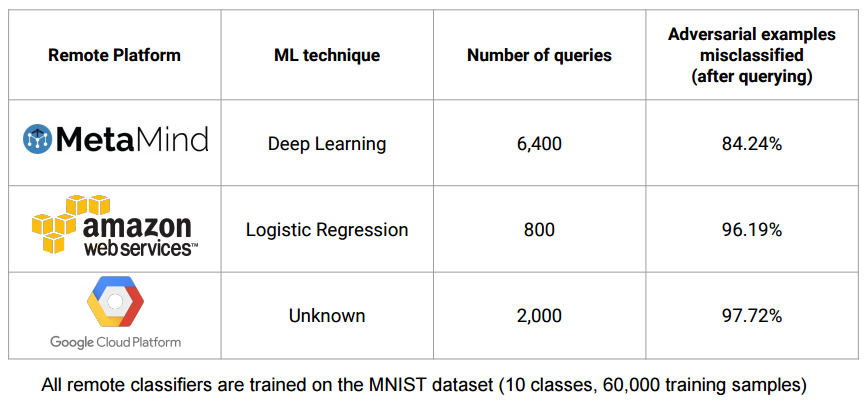
\includegraphics[scale=0.7]{black_box.png}
\caption{Black-Box attacks results against real world systems}
\label{tbl:black_box}
\end{table}

\section{Unrecognizable Images}\label{subsec:unrec}

Adversaries, on the other hand, are not restricted to small perturbations on known images. Nguyen et al (2015) presented a method for producing images that are unrecognizable to humans, but are nonetheless labeled as recognizable objects by DNNs \cite{nguyen2015}. For instance, a DNN would classify a noise-filled image crafted using their technique with high confidence. These images were named $fooling images$ since they do not have a source class but are crafted solely to perform a targeted misclassification attack.

\begin{figure}[!h]
	\centering
	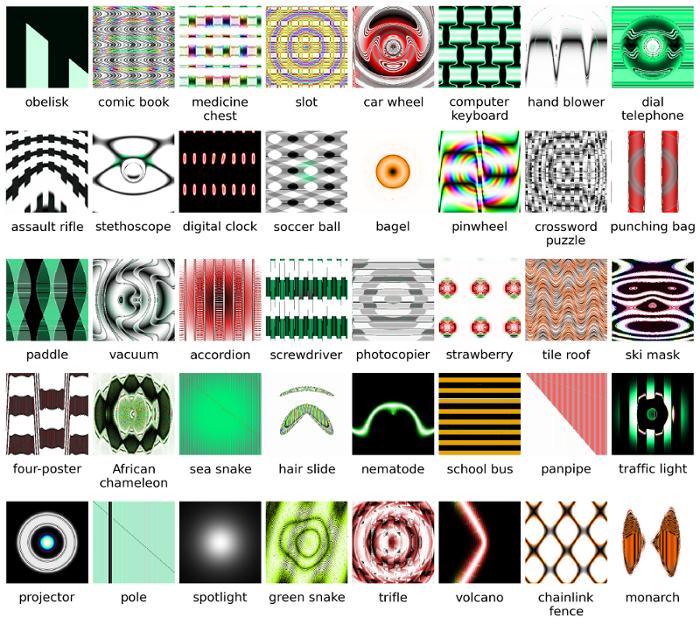
\includegraphics[scale=1.]{unrec_images.png}
	\caption{Examples of noisy images classified with high confidence \cite{nguyen2015}.}
	\label{fig:unrec_images}
\end{figure}


\section{Adversarials in the Physical World}\label{sec:physical}

All the aforementioned techniques rely on feeding information directly into the targeted machine learning systems. Such models only takes into consideration situations in which attacks take place entirely within the computer. For instance, these techniques could be used by attackers to avoid spam filters or malware detectors. Even though the study of adversaries in the digital world is utterly relevant, a recent study conducted by \cite{goodfellow2016} have shown that it is possible to craft adversarial samples so as to perform attacks on machine learning systems which are operating in the physical world.

Although the Fast Gradient Sign method have been successful on crafting adversarial examples, there are some extensions of the method that can be used in order to create perturbations that are more likely to work in the physical world. Goodfellow et al (2016) introduced a variation of the perturbation method named \textit{Basic Iterative Method}. This technique applies the fast gradient method multiple times with small step sizes and makes sure that all pixels are within a $\epsilon$-neighbourhood of the original image. The number of iterations was chosen heuristically with goals of being sufficient enough to have the adversarial example reaching the edge of the $\epsilon$ max-norm.

In order to create a physical world setting in the experiment, clean photos of adversarial examples created using the three methods were taken and fed into a machine learning system using Deep Convolutional Neural Networks (Inception V3). Adversarial Images created using the "fast" method were more robust when compared to the iterative methods. The hypothesis behind the result is that iterative methods create more subtle perturbations that can be easily be destroyed by the photo transformation process. Overall, it could be expected that about 2/3 of the images would be top-1 misclassified and about 1/3 top-5 misclassified by the fast method using an $\epsilon$ of 16.

Adversarial examples is not only feasible on digital attacks but also on physical world scenarios. By using the correct perturbation algorithm with optimized hyperparameters one can use printed digital photos to fool day-to-day machine learning systems. As more and more machine learning is becoming part of our environment, techniques for avoiding such attacks need to be developed so these systems can become less vulnerable to any kind of attack.

\section{Defending Against Adversarial Attacks}\label{sec:robustness}

Since adversarials are exploiting intrinsic network properties, these could also be used when training a network in order to develop robustness to possible examples crafted using the same methods. By using the worst case perturbation of a point \textit{x} instead of \textit{x} itself it is possible to derive an equation that includes the perturbation within its objective function. This form of training was able to reduce the error rate of adversarial examples from 0.94\% to 0.84\% \cite{goodfellow2014}. Adversarial training can be seen as a way of teaching the model how an adversarial looks like and that it should be able to generalize not only normal images but also perturbed ones. Another way of creating robustness was developed by using bayesian non-parametric methods. Estimating the confidence that an input is natural during the training phase can lead the network to generate priors that take into account adversarial perturbation of points \cite{billovits}. 

$$ C(\omega,x,y) = \alpha C(\omega ,x,y) + (1-\alpha )C(\omega ,x+\epsilon sign(\nabla_{x}C(\omega,x,y))$$

Most adversarial construction techniques use the gradient of the model to make an attack. In other words, they look at a picture of an airplane, they test which direction in the picture space makes the probability of the "cat" class increase, and then they give a little push in that direction. These are hard to defend against because it is hard to construct a theoretical model of the crafting process. These examples are solutions to an optimization problem that is non-linear and non-convex for many ML models, including neural networks. Since there is no good theoretical tool for explaining the solutions of these complicated problems, it is very hard to make any kind of theoretical argument that a defense can improve an algorithm from a set of adversarial examples.
\chapter{Experiment}

This chapter presents the experimental environment used during the development of this work. The first two sections will focus on discussions around the choices of data domain and the CNN architecture. The next section explains all the networks variants, techniques and parameters used during the training process. The two subsequent sections are dedicated to explain the reasons behind the chosen perturbation method and the synthetic generation of the imbalanced dataset, which are the core ideas behind this work.
\section{Data domain}

Advancement on Computer Vision were made possible by two driving forces: increased computational power and standardized datasets for benchmarking. The ever increasing amount of image data on the Internet fostered more sophisticated and robust algorithms to work on images and multimedia data. ImageNet is a large-scale ontology of images with 1.000 different classes and with 3.2 million 224x224 high resolution images in total \cite{deng2009imagenet}. CIFAR, on the other hand, is a more compact dataset with 32x32 colour images in 10 or 100 classes. The dataset consists of 60.000 images with equal amount of samples per class \cite{krizhevsky_2009}.

Even though the two datasets differ on image sizes and number of class labels, they share similar data domain. CIFAR can be seen as a subset of ImageNet dataset, therefore, convolutional filters from the latter could be used to improve performance of the former as shown by Yosinski et al.(2014). Our experiment uses a CIFAR10 full dataset on a adapted VGG16 architecture.

\section{The VGG Architecture}

As described in Chapter 2, a ConvNet is a sequence of layers where every layer transforms one volume of activations to another through a differentiable function. Three main types of layers are used to build these networks: Convolutional Layer, Pooling Layer and Fully-Connected Layer. A Convolutional Layer computes the output of neurons that are connected to local regions in the input, the Pooling layer performs down-sampling operations along the spatial dimensions of the input and, finally, the Fully-connected layer computes the class scores of the classifier. The chosen architecture should have enough layers for learning good features from the training set domain. For instance, a ConvNet Architecutre for CIFAR-10 could have the following configuration: [INPUT - CONV - RELU - POOL - FC].

Network architectures with higher accuracies have better generalization over the overall data input domain, however, adversaries are efficient into extrapolating the given domain by going to previously unseen regions of space (known as domain shift \cite{papernot2016}). For this work we had to make a choice of which network architecture would not only provide reasonable accuracy for our selected data domain (CIFAR-10) but would also be reasonable on the resource consumption. This way we can reproduce the requirements of a real world system where not only accuracy is taken into account when selecting a deep learning model.

From all networks tested on Canziani et al (2016), the VGG16-19 from Simonyan et al. (2014)  seemed to have the best trade off between accuracy and performance (inference time). The VGG architecture won the first and second places on the ILSVRC-2014 submission on the localisation and classification task.The main contribution of the VGG network was showing that the depth of the network is a critical component for good classification performance. The model can be assembled with 16 or 19 Conv/FC layers and it features an extremely homogenous architecture that only performs 3x3 convolutions and 2x2 pooling from beginning to end.

\begin{figure}[!h]
	\centering
	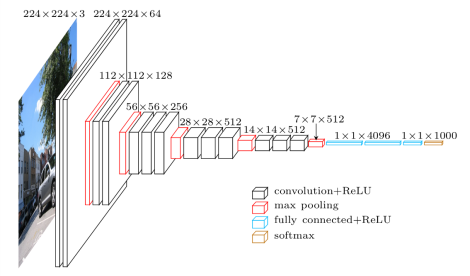
\includegraphics[scale=0.6]{imagenet_vgg16.png}
	\caption{VGG16 on ImageNet}
	\cite{simonyan2014very}
	\label{fig:vgg16}
\end{figure}

The design of the VGG16 has been proven to work even on datasets with several classes that are very different from each other . The two last fully connected layers of the state of the art model are comprised of 4096 neurons each, leading to much higher parameters complexity. As the dataset used in this work has only 10 classes, the two FC-4096 layers were replaced by one single layer with 512 neurons and RELU activations. This change helped to reduce overfitting when training the network. In addition, the total number of convolutions blocks and pooling were reduced to 3, with the first layer having 2 stacked convolution layers followed by a max pooling of stride 2x2 and the last two layers with 3 stacked convolutions also followed by a max pooling of stride 2x2. The max pooling layers are responsible for reducing the image size by 50\% every time an image passes through it. Since CIFAR-10 images are only 32x32, the original VGG16 architecture would end up having an output of shape of only 1x1 pixel at the last layer. In order to avoid this problem, the number of layers were reduced so to fit our dataset domain. The resulting shape fed into the fully connected layers is 4x4x128 (Width x Height x Channels) as it can be seen on table ~\ref{tbl:vgg10}. 

\begin{table}[!h]
	\centering
	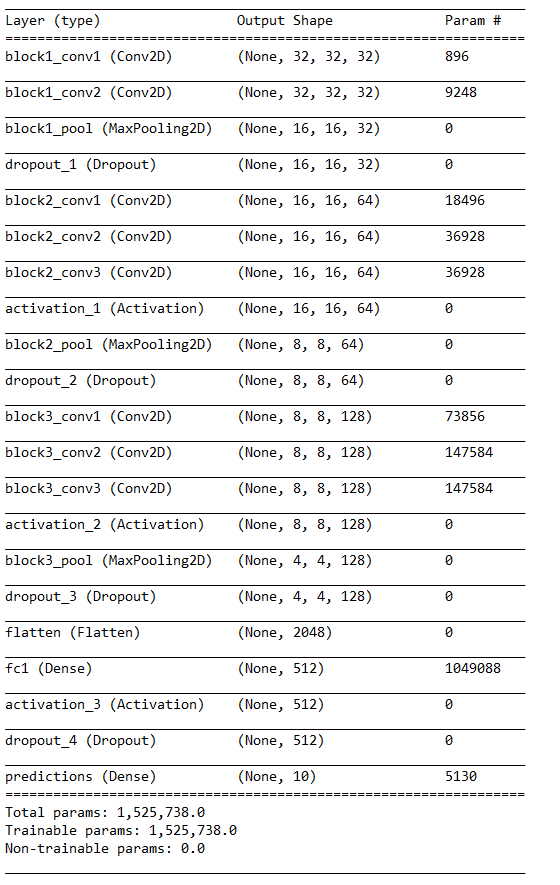
\includegraphics[scale=0.9]{vgg_arch.png}
	\caption{Full Model Description}
	\label{tbl:vgg10}
\end{table}
 
\section{Overall Training Process}

Neural Networks require good optimisation methods in order to achieve good performance. As networks get deeper, the number of resources required to train increases considerably. Convolutional Neural networks  can share parameters within its convolution layers, thus, reduce the amount of computation needed during training. All the models comprised in this work were implemented using Python programming language along with Tensorflow and Keras frameworks. The first is a high performance calculation engine that uses GPUs to accelerate its matrix/vector calculations. The latter is a Neural Network library that helps on the implementation of any deep learning model. Keras is mainly a wrapper on top of tensorflow that hides some abstraction from the developer, making it one of the best frameworks for DNNs currently.

As discussed on Chapter 2, the full gradient update would not be the best choice for optimizing deep networks. Stochastic Gradient methods were one of the first methods developed to overcome this problem and are still being further developed nowadays. The SGD based optimisation technique used in this work was developed by Bengio (2015) \cite{bengiormsprop}, namely RMSProp. This method is an adaptive learning rate scheme that can take the absolute values of the Hessian's eigenvalues and, therefore, approximate the equilibration pre-conditioner. As shown on Bengio's work \cite{bengiormsprop}, the method outperforms current SGD methods by achieving convergence faster.The learning rate for the method was set at $10^{-4}$ and the decay $10^{-5}$.

In order to achieve stability, every algorithm should be trained until convergence, in other words, it does no under-fit or over-fit the given dataset. Avoiding over-fitting and under-fitting is highly important when training DNNs. Our architecture was trained until no more reasonable changes were detected in the validation loss so we could dismiss unnecessary training steps and consequently any kind of over-fitting. This was achieved by using the Early Stopping technique as described on \cite{stanford2016}. Fundamentally, this consists of a functional callback that runs at the end of every epoch and compares the previous loss with the current one and interrupts training if the difference was below an user provided $\delta$ for a specific number of steps in a row. The value of our $\delta$ was set at $10^{-4}$ and the number of steps to 10. For instance, training would be stopped if no improvement over the specified $\delta$ was seen for 10 steps in a row. Also, we did put a hard limit of 200 on the total number of epochs.

\begin{figure}[!h]
	\centering
	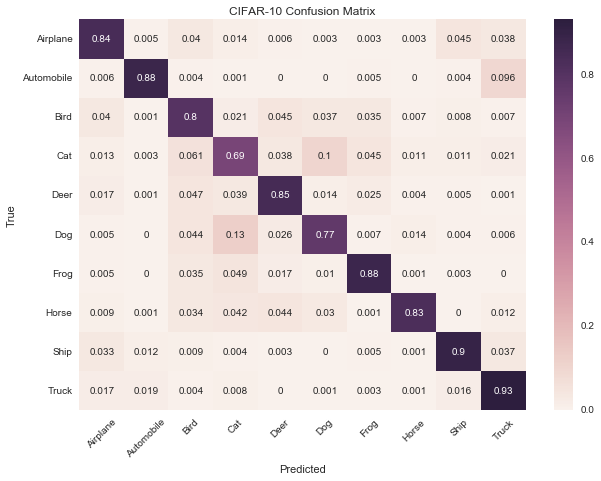
\includegraphics[scale=0.6]{conf_matrix.png}
	\caption{Results on the full dataset}
	\label{fig:conf_matrix_full}
\end{figure}

The confusion matrix helps understanding the individual score for each class and also which targets class were being misclassified into. Figure ~\ref{fig:conf_matrix_full} shows that the Cat and Dog classes are often interchangeably misclassified as they have a set of similar features. The network have reached an overall accuracy of 83.45\% and a total validation loss of 0.5033.

\section{Perturbation method}
Section ~\ref{sec:gsm} has shown two different types of perturbations that could be applied to images in order to generate adversaries. For instance, one could select a specific class as the target of a perturbation but this would ultimately introduce undesirable variance when crafting adversaries, as each class could have different effects within our target and, thus, the perturbation could be different on each case. In order to address this problem, we have chosen the class itself as the backpropagated gradient coupled with the ascent method. The intuition behind this choice is that we look to increase the cost function of the target class by moving away from the current label. As the class itself is chosen to cause the perturbation, our method moves to the closest data domain to our class, in other words, it follows the class own gradient uphill. For instance, cats and dogs are classes with similar feature spaces and are often misclassified among each other. A small ascent perturbation on any of these classes would likely lead to an increase on this prior effect as both classes are occupying similar positions of the space. 

For all classes, the amount of change on each pixel needed to be carefully chosen as we did not want to change an image too much to a point where it would be unrecognizable to human perception. Moreover, in order to test our networks, we needed an $\epsilon$ value that would provide only the minimum amount of perturbation to all classes so as to push most of the samples to the closest vicinity leading to a successful misclassification. From all the trials, the value of $\epsilon$ that seemed to fulfill our needs was 0.01. Another important choice was regarding which trained network would serve as the baseline for our gradient calculation. We have generated perturbation using two different networks on each of the 10 classes. We first generate one model for each class using both undersampled and oversampled datasets. Then for each of these models we created adversaries using its own current model and the balanced network. The balanced network itself was also tested using its own adversaries on all 10 classes at once to serve as baseline for our comparison. From now on we call this same model pertubation and different model pertubation, each being subdivided into the undersample and oversample case.

\section{Synthetic data level imbalance}

Classification models are usually required to have similar number of samples for each class in order to equally learn proper feature representations for each label. As shown on Murphey and Guo (2004) \cite{murphey2004}, Neural Networks have lower generalization capabilities and are biased towards specific classes when trained on datasets with unequal number of samples between classes. 

As the CIFAR10 dataset is not naturally imbalanced, we have artificially created two variations on which we trained our networks.  While one dataset consisted on a direct undersample of the target class to 1,000 samples, the other was crafted using  an oversampling of the target class(or an undersampling of all other classes). We kept the number of samples for the target class at 5,000 while all other classes was reduced to 1.000 samples each. For each class of the 2 different dataset configurations, a network was then trained until convergence using the same hyper-parameters as the balanced case. Each model was evaluated against a test set of 10000 equally distributed samples with the target class being perturbed by 3 different networks. In summary, we have created adversaries using the balanced network, the undersampled and oversampled networks. Both imbalanced networks were separately tested for each class with adversaries being generated by its own model and by the balanced network. The same model test aims to understand the vulnerability of class imbalance on adversarial examples while the different model test main goal is to verify the robustness on transfer learning environments. In total we evaluated 50 different combinations: 20 for each different imbalanced dataset (same model gradient and balanced network gradient) and 10 for the balanced network using its own gradients on each class.

\begin{figure}[!h]
	\centering
	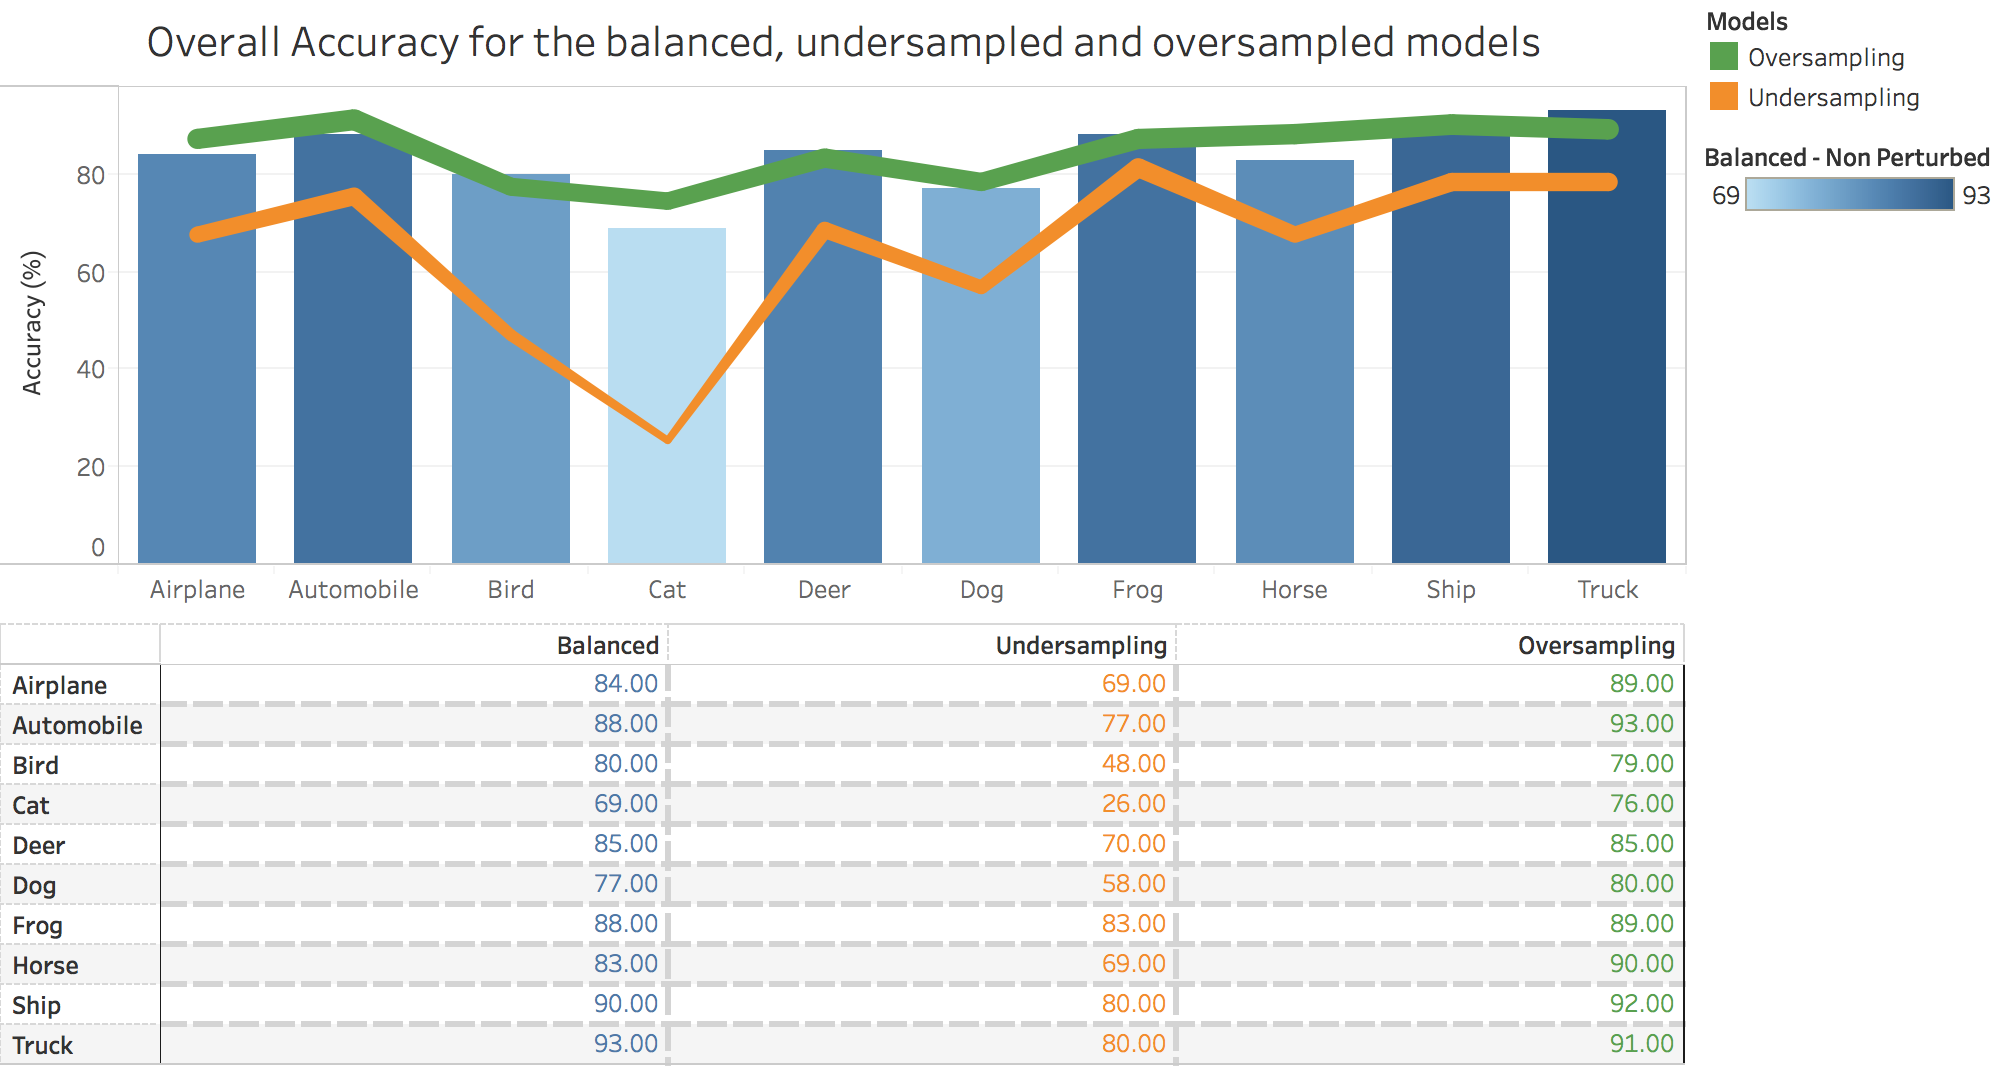
\includegraphics[scale=0.3]{graph_non_pert.png}
	\caption{Target class accuracy on all models}
	\label{fig:acc_graph}
\end{figure}

Figure ~\ref{fig:acc_graph} shows the per class accuracy for each specific model on non-perturbed test set. While the downsize on other classes causes the per class accuracy to increase, the downsize on class causes the same accuracy to be drastically reduced when compared to the balanced model shown on figure ~\ref{fig:conf_matrix}. The former happens because the model learns more about the target class due to its increased number samples, hence, it concentrates on learning the specifics of the class rather than equally splitting its capacity through all classes as it happens on the latter. The increased accuracy means that the model better explores the space around the target class since it does not have enough evidence to explore other classes spaces.

\section{Experiment goals}
This work focuses on explaining the relationship between the data imbalance learning problem and adversarial attacks. Both subjects relate to each other as they are different ways of explaining the underlying data space exploration by the machine learning method. As datasets go into higher dimension, it becomes harder to the human rational to explain space transformations, as one usually is able to visualize only smaller dimensions of space. Specifically deep learning models are seen as "black box" due to its high complexity learning behavior. We try to understand which adversarial attacks are more effective against models were the target class is both undersampled and oversampled. Moreover, we investigate situations where two or more classes have strong similarities and therefore share close spaces in the data domain, creating overlapping distributions. Lastly, we generate perturbation from a different model and we test it on the target model to understand the effect of transfer learning on imbalanced networks.



\chapter{Results}
In this chapter we show the results from our experiments on different types of imbalanced datasets. We first start by showing the results on the balanced model so as to set the baseline of comparisons. A discussion then follows on the under-sampled and over-sampled cases, ending with the transfer learning results for perturbations with different models. The chapter is then concluded with the results for the cases where classes have similar features, and, therefore, share overlapping distributions.


\section{Fully balanced model}

The objective of this research is to understand the effects of adversarial attacks on imbalanced CNNs. Canonical models assume that every object in the dataset are sampled from similar distributions. However, in real-life situations, even though the number of samples is the same, some class labels could be poorly represented by the lack of a clear structure. This could often lead to differences in the output for each specific class \cite{krawczyk2016learning}. On this way, a superficially balanced dataset does not guarantee that the model will equally generalise across all classes. Adversarial attacks were firstly done on a fully balanced model so as to use its results as baseline of comparisons for our imbalanced models.
\begin{figure}[H]
	\centering
	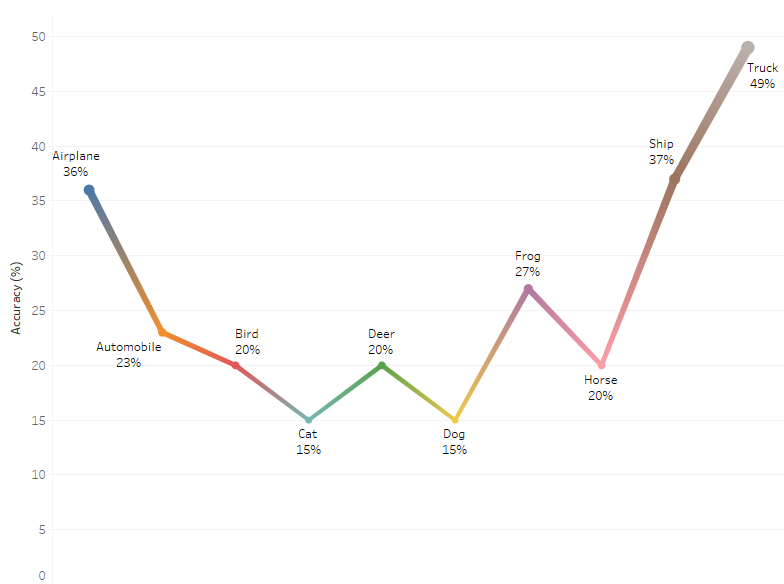
\includegraphics[scale=0.7]{balanced_perturbed.png}
	\caption{Individual class perturbed accuracy on the balanced model}
	\label{fig:balanced_perturbed}
\end{figure}

Figure ~\ref{fig:balanced_perturbed} shows that the accuracy for all classes is drastically reduced when the balanced model is presented with adversarial examples. Even though there is enough samples for each class, the adversarial attack forces the domain shift of each individual sample towards different regions in space, causing a misclassification of the current label. The effectiveness of the adversarial attack can be partially explained by the balancing of the dataset itself. In a model where the dataset used in training aims for normalization over all classes, the network is often caught in trying to find weights and biases that generalises well over all set of labels. Therefore, perturbations become more efficient due to a bigger proximity of classes distributions in space.


\section{Class under-sampling and over-sampling}


As the number of samples on a target class goes down, an increase of vulnerability towards that specific label is expected when compared to the balanced model. The results on table  ~\ref{tbl:results} confirms this. Networks with imbalanced datasets were more vulnerable when presented with adversarial examples. Figure ~\ref{fig:relative_difference} shows the relative difference for all the three networks (balanced, under-sampled and over-sampled).  The values were calculated by finding the difference between the new accuracy and the non-perturbed accuracy. They represent the percentage on which the initial accuracy was reduced. The under-sampled model had the higher relative difference on average, which shows that the imbalanced nature of the dataset ended-up increasing the vulnerability of the model. This poses threats to current systems as the low amount of samples during training for a specific class would  create gaps that are more easily exploited when compared to a balanced network. For instance, the decision boundaries of distributions are affected by the number of samples on the training set and, thus, can change model performance across each class.

Class imbalanced models are naturally affected by the false positive and false negative trade off shown on figure \ref{fig:class_dist}. The decision boundaries on such models favour the class with more samples and, hence, increases the accuracy for one class while decreasing for the other class. The area under the curve for misclassified examples on the under-sampled distribution is bigger, and it is caused by the suboptimal exploration of feature space of that class. This effect is exploited by adversaries as there is an increase on the misclassification rate of distributions with lower amplitude. An under-sample of a specific label causes its distribution to be squished into space and, hence, have less impact on the definition of decision boundaries.

\begin{figure}[H]
	\centering
	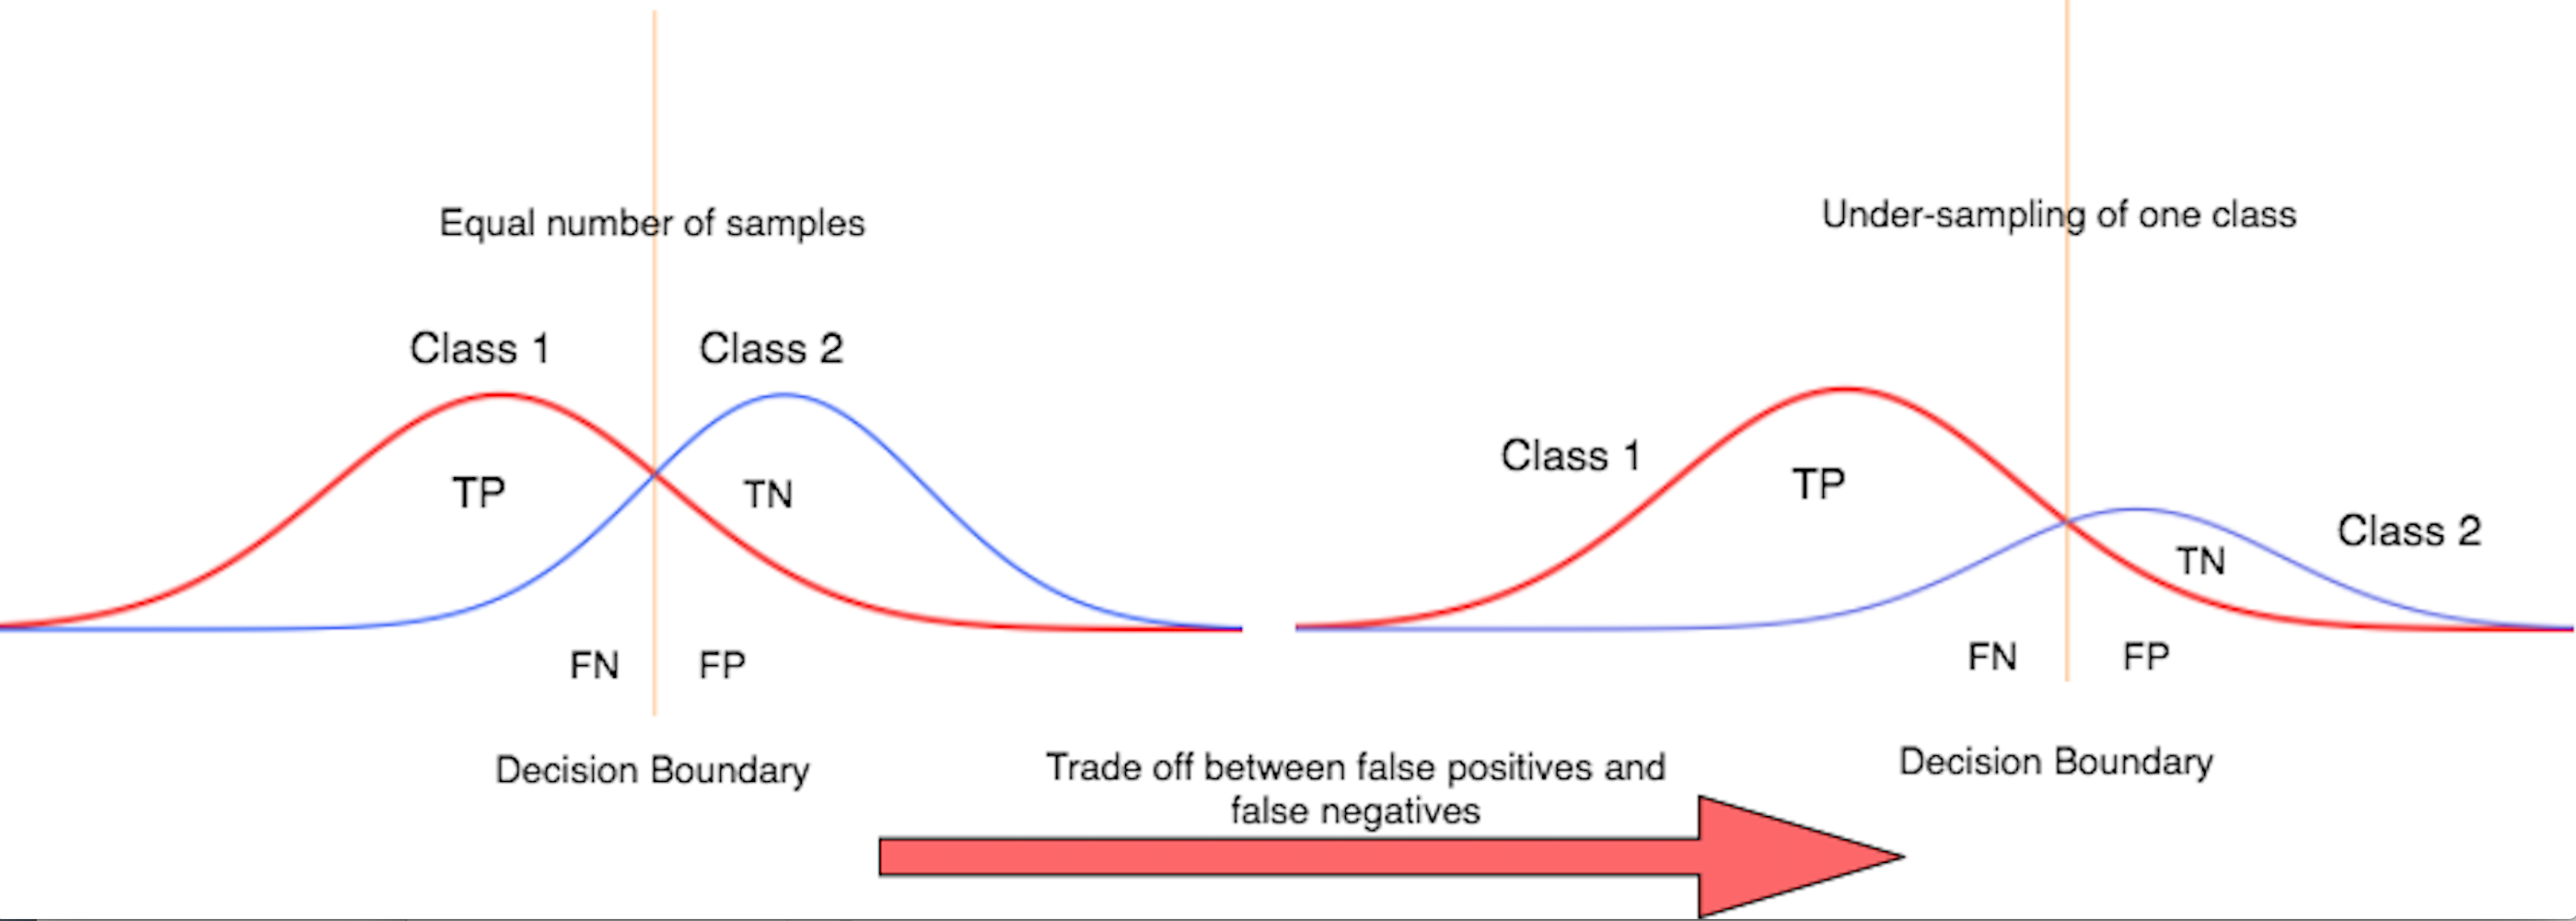
\includegraphics[scale=0.32]{class_dist.png}
	\caption{Dataset imbalance causes models to perform adjustments of decision boundaries leading to an increase on accuracy of the majority class and decrease on the minority class.}
	\label{fig:class_dist}
\end{figure}



\begin{table}[H]
	\centering
	
	\begin{tabular}{lccccc}
		\toprule
		&\multicolumn{2}{c}{Different Model}
		&\multicolumn{3}{c}{Same Model}
		\\\cmidrule(r){2-3}\cmidrule(l){4-6}
		Class Label &Undersample &Oversample &Balanced &Undersample &Oversample \\
		\midrule
		0 - Airplane &60\%& 87\% &36\%& 19\%    & 61\% \\
		1 - Automobile &64\%& 91\% &23\%& 16\%    & 63\% \\
		2 - Bird &38\%& 73\% &20\%& 9.4\%    & 27\% \\
		3 - Cat &21\%& 72\% &11\%& 0.5\%    & 19\% \\
		4 - Deer &58\%& 80\% &20\%& 9.8\%    & 20\% \\
		5 - Dog &47\%& 76\% &15\%& 9\%    & 38\% \\
		6 - Frog &76\%& 88\% &27\%& 20\%    & 49\% \\
		7 - Horse &59\%& 88\% &20\%& 18\%    & 52\% \\
		8 - Ship &69\%& 89\% &37\%& 19\%    & 59\% \\
		9 - Truck &46\%& 87\% &49\%& 21\%    & 54\% \\
		\bottomrule
	\end{tabular}
	\caption{Results for the two different sources of perturbations along with the two different imbalanced datasets}
	\label{tbl:results}
\end{table}

On the over-sampling case, the classes with more samples will naturally have higher overall influence when compared to classes with lower number of samples. This happens as the network performs more gradient updates on that specific class due to the amount of available samples. Perturbation on this case had a lower effect, as the small push caused by our $\epsilon$ was not enough to move points to outside of their distributions. Objects of the over-sampled classes would need bigger steps in order to successfully create an adversarial that leads to a misclassification output. Accuracy for most cases of the over-sampling case was around 45\% and the relative difference was the lowest of all three models, which shows robustness towards the target class. This approach can be used to increase system robustness on a specific label. For instance an application could have the desire to make a class stronger than the others due to critical factors on the classification of that label.

The increased number of samples of the over-sampled label, causes the network to perform a trade-off when optimizing its loss function. For instance, the decision boundary would be chosen in order to minimize the total error of the network. The cost function is lower when the decision boundary minimizes the misclassification of the majority class, as there is a higher number of samples. This phenomenon is well explained by figure ~\ref{fig:class_dist}, as the intersection of both distributions causes the densities to be different when we change the dataset balance.

\begin{figure}[H]
	\centering
	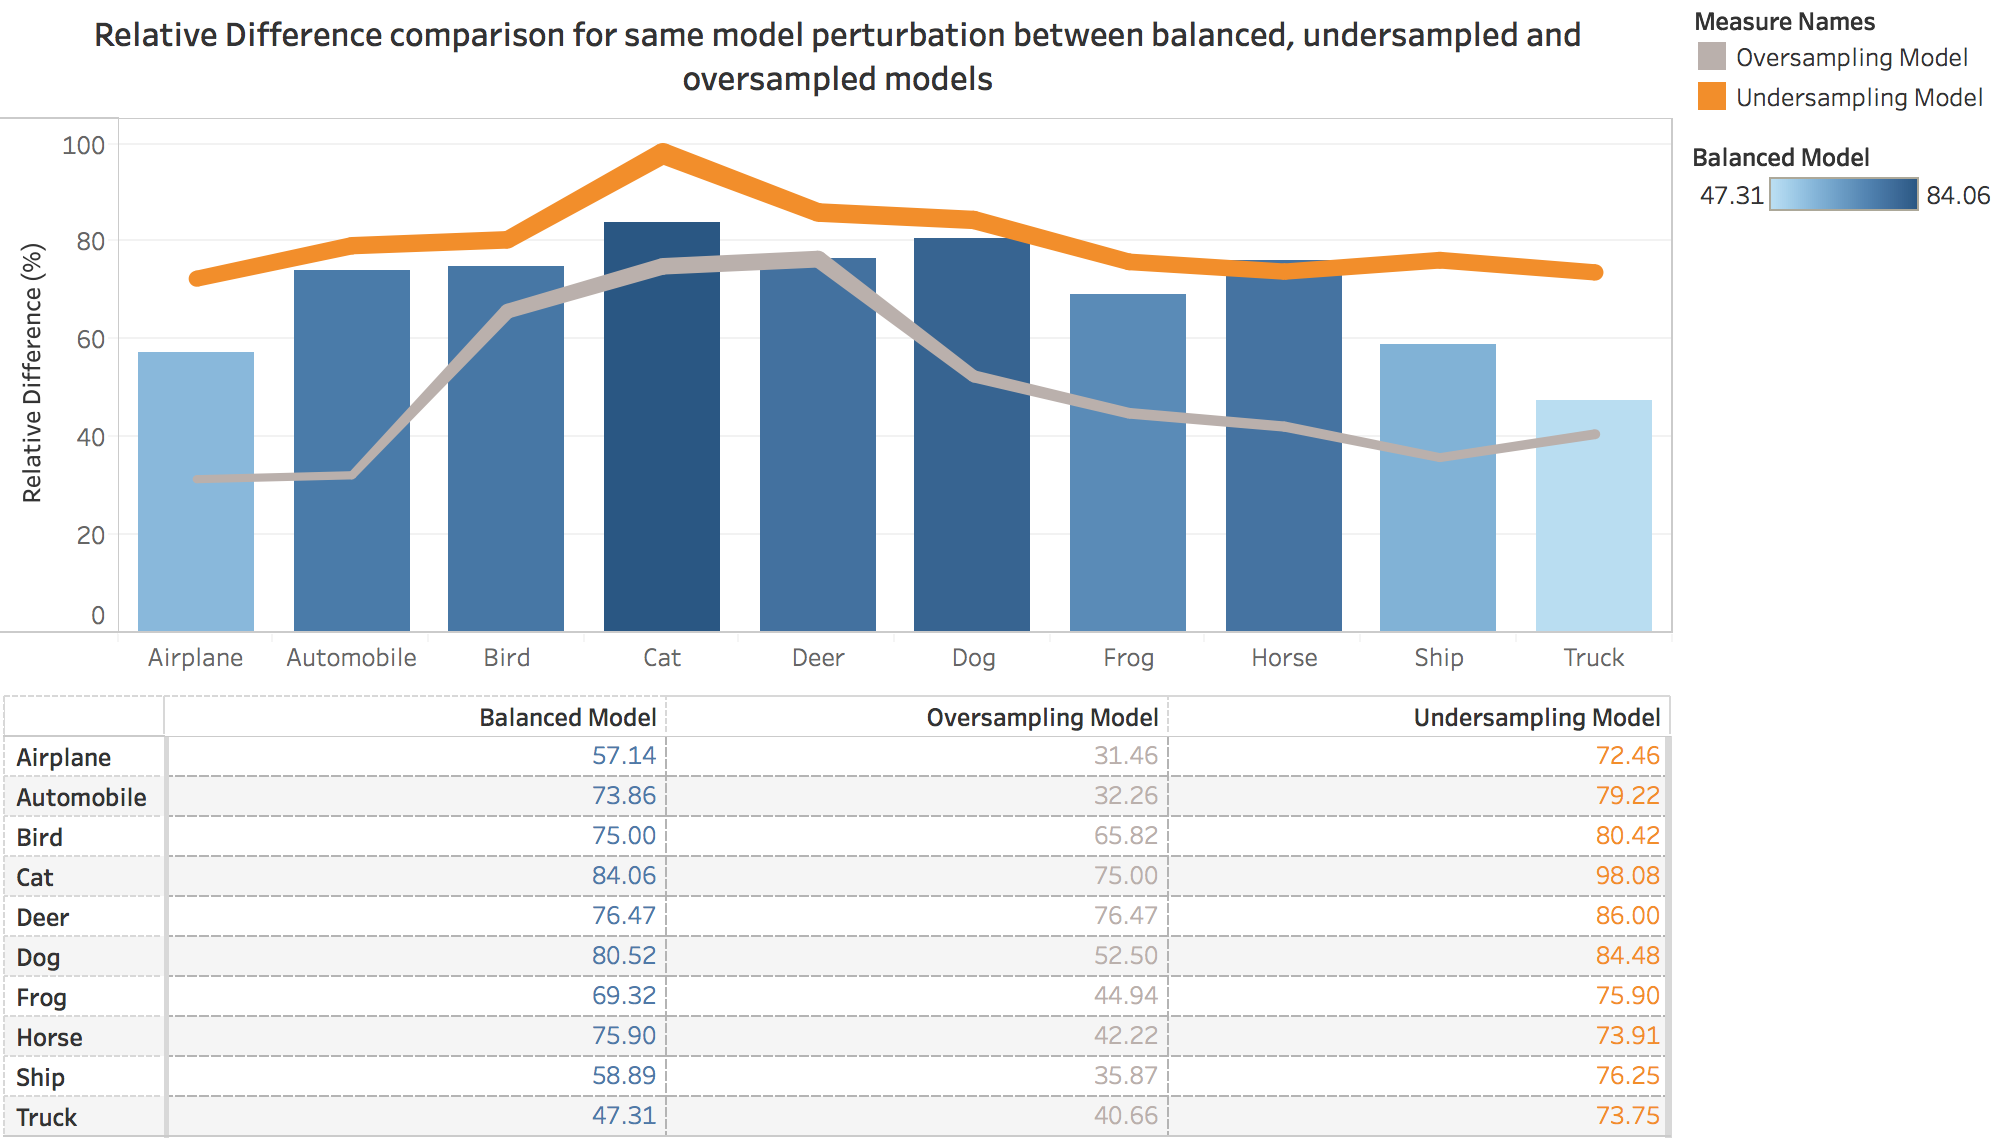
\includegraphics[scale=0.3]{rel_diff_graph.png}
	\caption{Relative difference for each model. Higher numbers means more vulnerability}
	\label{fig:relative_difference}
\end{figure}

\section{Transfer Learning}

Chapter 4 discussed different ways in which one algorithm could learn from existing models. When the attacker has no knowledge of the underlying model that he/she wants to attack, the best way to learn the gradient information is by querying the target and training a new model with its outputs. The use of a different model for creating adversaries has shown less effective when compared to the same model attack. As the overall gradient have not only different direction but also magnitudes, the attacked system has proven to be more robust. The experiment reveals that although Gradient Sign is quite effective for fooling networks it does require a good amount of knowledge from the underlying training parameters so as to unleash its full potential.

Attacking an under-sampled network with the gradient of the balanced network did not show to be as effective as using the same model's gradient. The average accuracy of an under-sampled model attack with adversaries generated from a different network was 53.8\% while the same metric was 25.8\% for the same model attack. Even that our training samples are within the same data domain, there are still huge differences on the gradients learned from the network. 

\section{Overlapping distributions}
When classes in the dataset already have distributions that are very close to one another the effects of adversaries seems to be even stronger. Figure ~\ref{fig:conf_matrix_full} shows that for the pairs cat and dog and automobile and truck, misclassification naturally happens towards one another due to similarities in their feature space \cite{stanford2016}. On this case, our experiment shows that the adversarial attacks intensifies this property by increasing the number on which one class is picked over another. Figure \ref{fig:overlap} shows that both cat and dogs are increasingly misclassified between themselves when imbalanced datasets on both classes are used. While on the cat under-sampling case 40\% of the samples were misclassified as dogs, on the oversampling 39\% of the dogs were misclassified as cats. This results gives interesting insights, as it shows that the gradient sign is navigating around the target class distribution and when an overlap occurs it becomes easier to create an adversarial to the class with higher similarities.

\begin{figure}[ht] 
	\label{fig7} 
	\begin{minipage}[b]{0.5\linewidth}
		\centering
		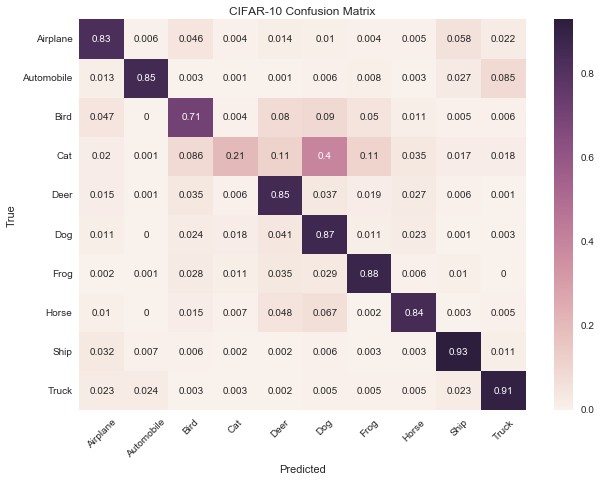
\includegraphics[width=1\linewidth]{cat_undersampling_per.png} 
		\vspace{4ex}
	\end{minipage}%%
	\begin{minipage}[b]{0.5\linewidth}
		\centering
		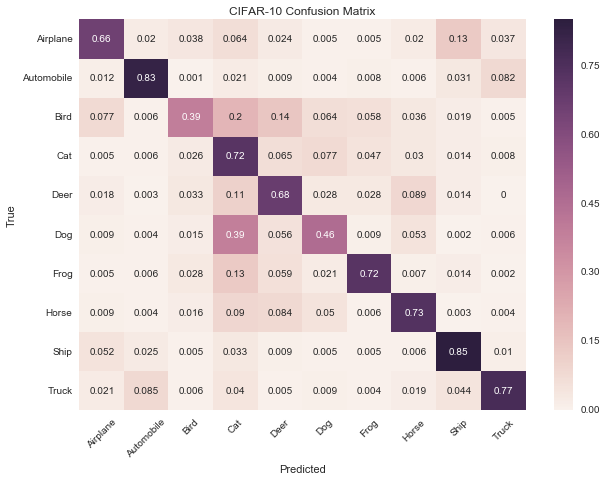
\includegraphics[width=1\linewidth]{cat_oversampling_per.png} 
		\vspace{4ex}
	\end{minipage} 
	\begin{minipage}[b]{0.5\linewidth}
		\centering
		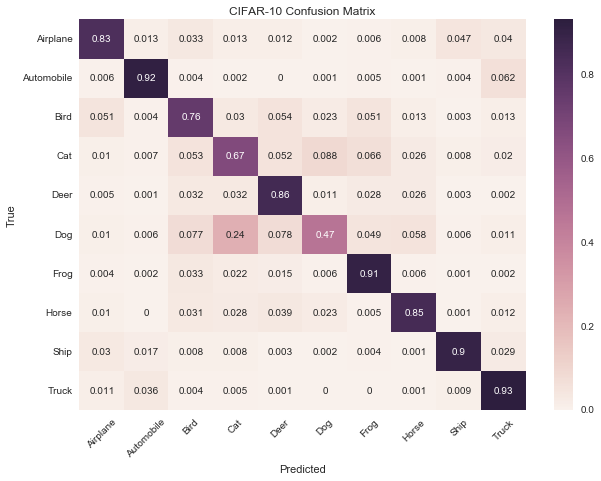
\includegraphics[width=1\linewidth]{dog_undersampling_per.png} 
		\vspace{4ex}
	\end{minipage}%% 
	\begin{minipage}[b]{0.5\linewidth}
		\centering
		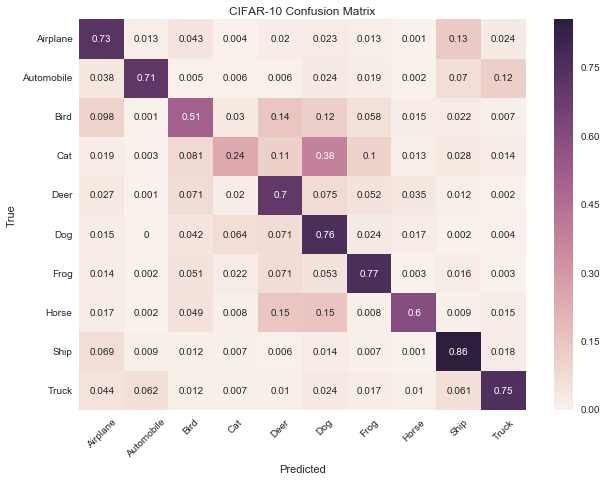
\includegraphics[width=1\linewidth]{dog_oversampling_per.png} 
		\vspace{4ex}
	\end{minipage} 
	\centering
	\caption{Top Left and Right: Cat undersampling / oversampling with perturbation. Bottom Left and Right: Dog undersampling / oversampling with perturbation}
	\label{fig:overlap}
\end{figure}

Classes with overlapping distributions sheds some light on the effect of the $\epsilon$ value of the gradient sign method. Its clear to understand that classes that are close together in the data space are required to take smaller steps in order to be successfully misclassified. Both dog and cat classes were already being confused with one another before the adversarial attack, and the small "push" of the gradient method has increased this effect, showing that domain shift is even stronger on these situations. The required amount of steps for classes with high level of uncertainty around them is often smaller when compared to classes with a better and more confident exploration of space.
\chapter{Results}

In this chapter, we present approaches for attacking machine learning algorithms with adversarial techniques presented in the previous chapter. We discuss that the knowledge of the architecture and weight parameters is sufficient to derive adversarial samples against DNNs. Further discussion goes into black box attacks where the attack has minimal information about the underlying system. The discussion is then closed with how model's knowledge can be transferred between different algorithms/techniques.

\chapter{Conclusion}

Adversarial methods are proven to increase the domain shift effect on test datasets as it is explained by Papernot et al (2016) \cite{papernot2016transf}. Yet, one should be careful when trying to interpret this shift without actually understanding how the feature space was actually explored. The imbalanced learning problem is not intensified by Adversaries created with the same class gradient. It should be noted that the effectiveness of the method dependence is twofold: how strong a specific class gradient is on the overall dataset and the space occupied by its distribution in space.

The right relationship between gradient strength and target class distribution is what causes networks to misclassify examples. A strong enough gradient would mean bigger steps towards other distributions and a small gradient would not have enough strength to move points from outside of their distributions. In order to keep perturbation constants across different models, one would need to tune $\epsilon$ accordingly in order to generate images with the lowest amount of noise possible and still get a successful attack. Until now, most of the studies in adversaries were aimed in created methods that could effectively create those perturbations, however, one should aim to understand its characteristics more deeply as this not only helps to understand networks vulnerabilities but also provides new tools to explain the "black box" effects of deep neural nets. The answer to our major hypotheses are as follows:

\begin{itemize}
	\item \textbf{(H1)} - Adversaries still reduce the overall accuracy when compared to a fully balanced model, but in a lower degree when compared to the same perturbation applied to a model trained without any form of imbalance
	\item \textbf{(H2)} - The effects on this case are almost negligible, the networks were able to resist attacks really well, and the average reduction of accuracy was around ~1-2\% on most cases
	\item \textbf{(H3)} - Attacks on classes with overlapping distributions do intensify the natural behavior, as this situation really opens the ideal vulnerability adversaries are looking for.
	\item \textbf{(H4)}
\end{itemize}

This work sheds an important light on machine learning methods. Several real-life models are deeply concerned with possible vulnerabilities of their system, and studies on this field were being done for the past 20 years. Still, the imbalance learning problem remains one of the big questions in artificial intelligence. Adversarial attacks are one more concern for those working with such systems, but could also be seen as a tool that could forcibly make a model to stretch its occupation over the data domain space. Every new threat to predictive techniques is also a new improvement over model generalisation capabilities as the creation of the former could be used to improve the latter. Imbalanced datasets can be seen as one way of avoiding adversarial attacks, as the both lack and extreme excess of data space exploration seems to increase models robustness to such attacks

\section{Future Work}

%now enable appendix numbering format and include any appendices
\appendix
\chapter{Sample Title}

Lorem ipsum dolor sit amet, consectetur adipiscing elit, sed do eiusmod tempor incididunt ut labore et dolore magna aliqua. Ut enim ad minim veniam, quis nostrud exercitation ullamco laboris nisi ut aliquip ex ea commodo consequat. Duis aute irure dolor in reprehenderit in voluptate velit esse cillum dolore eu fugiat nulla pariatur. Excepteur sint occaecat cupidatat non proident, sunt in culpa qui officia deserunt mollit anim id est laborum.
\chapter{Sample Title}

Lorem ipsum dolor sit amet, consectetur adipiscing elit, sed do eiusmod tempor incididunt ut labore et dolore magna aliqua. Ut enim ad minim veniam, quis nostrud exercitation ullamco laboris nisi ut aliquip ex ea commodo consequat. Duis aute irure dolor in reprehenderit in voluptate velit esse cillum dolore eu fugiat nulla pariatur. Excepteur sint occaecat cupidatat non proident, sunt in culpa qui officia deserunt mollit anim id est laborum.

%next line adds the Bibliography to the contents page
\addcontentsline{toc}{chapter}{Bibliography}
%uncomment next line to change bibliography name to references
%\renewcommand{\bibname}{References}
\bibliography{refs}        %use a bibtex bibliography file refs.bib
\bibliographystyle{plain}  %use the plain bibliography style

\end{document}

